\section{展望：通往物理通用人工智能之路}
\label{sec:path-to-physical-agi}
大语言模型（LLM）使机器以前所未有的程度掌握了人类语法、语义和积累的知识。然而，尽管大语言模型对我们如何描述现实有百科全书般的理解，它们却缺乏对物理现实本身的根本依托。我们正在迅速接近离身智能的极限\citep{coveney2025wall}。

语言模型与世界模型的关系，定义了人工智能发展的下一次重大范式转变。要勾勒通往通用人工智能（artificial general intelligence，AGI）的更广阔道路，必须认识到人工认知的一个基本事实：i）语言赋予机器谈论世界的方式；ii）世界模型将使机器理解世界、想象世界、借助世界进行推理，并在其中行动。如果AGI需要在物理领域导航和操作，就不能只靠预测序列中的下一个词完成这些任务。它必须原生地具备对物理、因果、空间推理和时间的直觉理解，必须能够在行动前模拟后果——预测现实本身的下一个状态；更重要的是，它需要评估给定当前物理智能体，在真实世界中哪些任务可能实现。

\paragraph{三位一体架构：自主演化的引擎}
要实现物理通用人工智能（Physical AGI）愿景，仅有基于历史数据被动训练的静态模型还不够。AGI需要一个动态、自我演化的系统，能够持续与真实世界交互并自主学习。为此，我们提出\textbf{三位一体架构（Trinity Architecture）}这一概念：一个三部分的认知循环，旨在自主弥合数字推理与物理能力之间的差距。架构由三个相互依赖的组件构成：
\begin{itemize}
\item \textbf{智能体（Agent）：任务执行引擎。}行动者（Actor）即物理智能体，接收任务指令，并以物理方式（或物理模拟方式）尝试完成任务。它将高层意图转化为环境中细粒度、序贯的行动。
\item \textbf{评估器（Evaluator）：任务完成的裁判。}智能体运行时，评估器观察轨迹数据，评价任务完成的有效性与效率，对失败、物理规律违反或次优运动提供精确反馈。
\item \textbf{世界模型：核心模拟器与课程设计者。}世界模型接收智能体生成、经评估器评分的轨迹数据，通过观察交互，学习世界的底层物理、动力学和因果关系。关键在于，世界模型理解智能体当前能力的确切\emph{边界}，利用内部模拟，想象并提出复杂程度逐渐提高、\textit{略超出}智能体当前能力的新任务，充当自动课程生成器。
\end{itemize}

这里，世界模型承担关键角色：i）内化世界知识；ii）了解当前行动者可行任务的边界；iii）通过提出新任务，指导下一轮智能体—世界交互。这也类似于人类学习和使用脑内世界模型的方式\citep{taniguchi2023world,deng2025simura}。行动者与评论家组件同样可以借助大语言模型增强，例如实现为基于大语言模型的多智能体系统\citep{yang2025unlocking}；因此，这些组件中的规划、推理与决策，自然依赖大语言模型的认知智能。由此，三位一体架构提供了大语言模型与世界模型相互增强的机制。

\begin{figure}
    \centering
    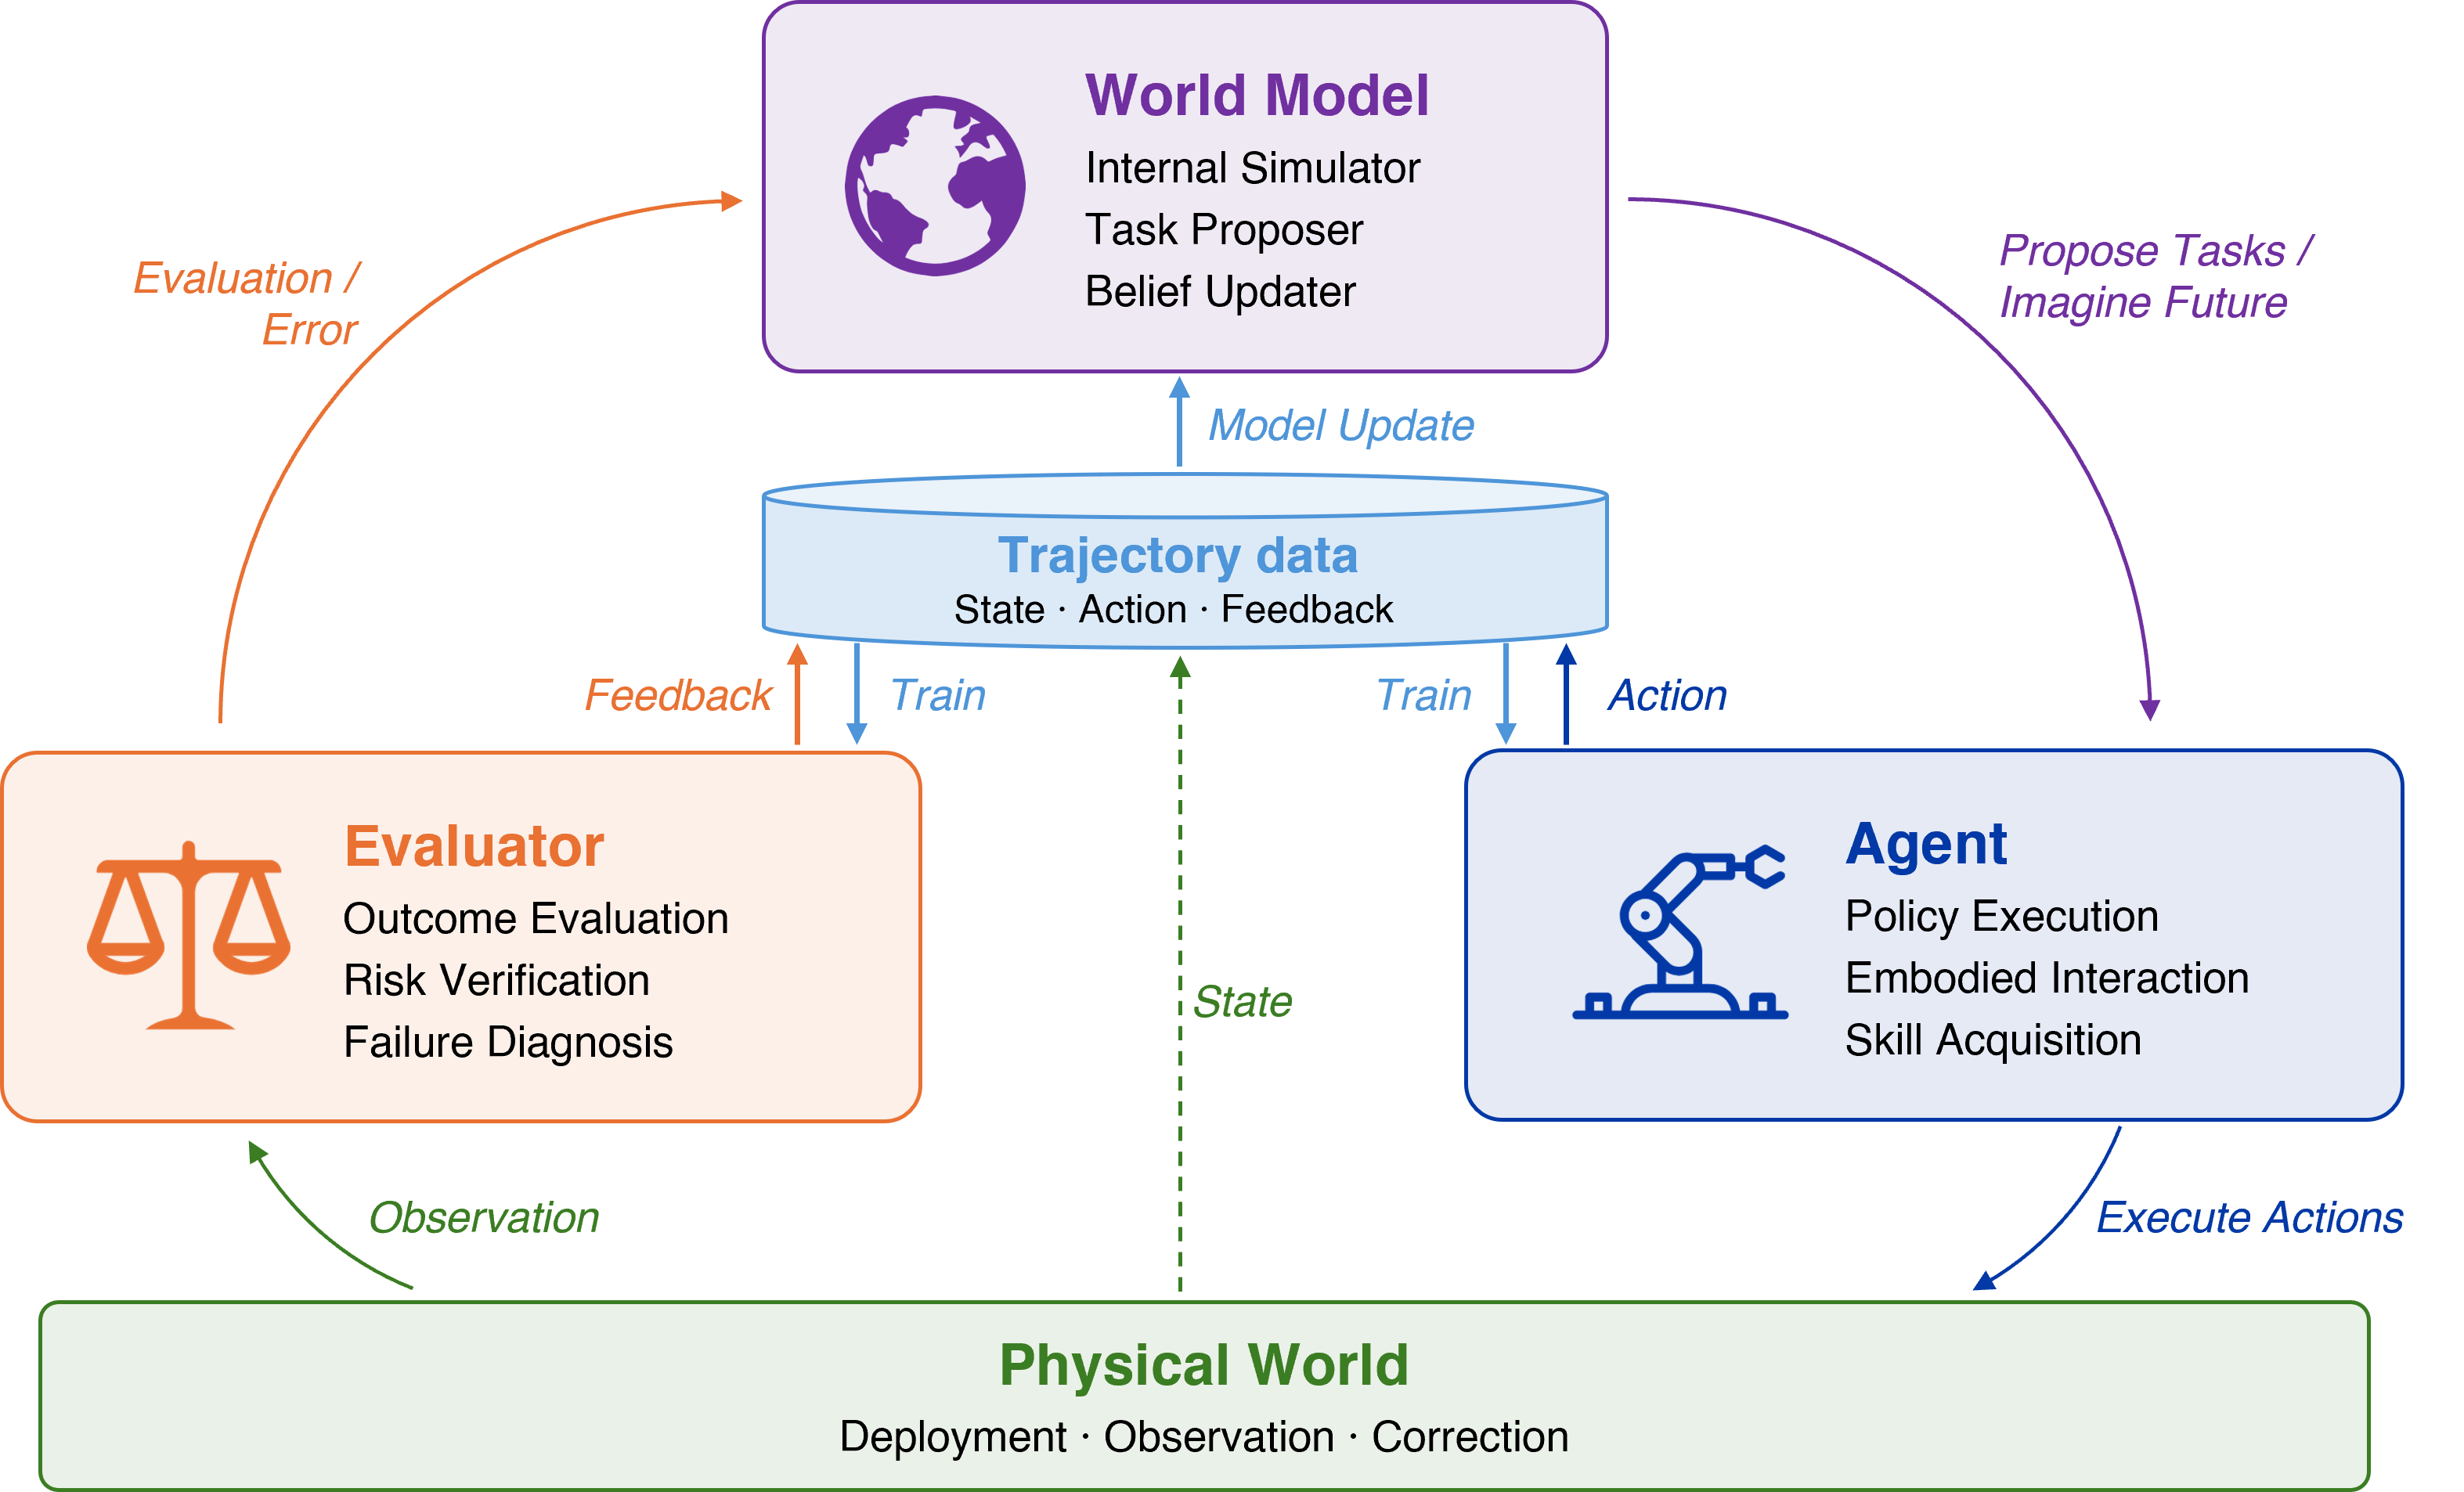
\includegraphics[width=0.85\linewidth]{figs/trinity_architecture2.png}
    \caption{三位一体架构概览。}
    \label{fig:trinity}
\end{figure}

\paragraph{通过与世界交互迈向AGI}
这一三位一体体系的真正力量，在于与现实持续交互。循环同时运行于数字模拟与物理世界。世界模型可以安全地想象数千种情境，并提出任务，让行动者先在高保真数字孪生（digital twin）中尝试。行动者掌握这些任务后，系统将所学直觉部署到物理世界，评论家评估现实中不可避免的摩擦与噪声，再将新数据反馈给世界模型。

通过不断行动、评估和更新内部模拟的循环，人工智能不再完全依赖人工整理的数据集，而开始像生物智能一样，通过物理试验、错误和想象来学习。这一三位一体架构不仅是改进机器人的蓝图，也是将人工智能从被动对话者转变为主动的物理AGI的演化引擎。
